\section{Shape index and query-shape containment}

\sepfootnotecontent{shapetrees}{
    \href{https://shapetrees.org/TR/specification/}{https://shapetrees.org/TR/specification/}
}

\sepfootnotecontent{fn:solidPrivacy}{
In this work, we do not take into consideration confidentiality restrictions.
}

\sepfootnotecontent{fn:litShapeComparaison}{
There exist comparisons between the shape and class definition approaches in the context of data validation~\cite{demeester_swj_2021} but it is left to be determined if their frame of comparison is compatible with our current problem
and foreseen opportunities.
}

The RDF specification does not enforce schemas on data.
However, the data published often adhere to an implicit schema due to the nature of the data and the formulation of RDF~\cite{Neumann2011CharacteristicSA}.
Implicit schemas have been used for query optimisation~\cite{Neumann2011CharacteristicSA, Meimaris2018HierarchicalCS}.
We propose to adapt those methods for LTQP by using explicit data schemas provided by the data provider in our source selection process.

The goal of the shape index is to reduce the query execution time by minimizing the dereferencing of unnecessary RDF documents in subdomains of the web (set of URL or URL patterns).
We define a shape index as a set of mappings between RDF data shapes and sets of resources.
This mapping concept shares similarities with shape mapping~\cite{Gayo2018} and target declarations~\cite{Gayo2018Shacl}.
However, instead of mapping shapes to RDF subgraphs, it maps shapes to sets of documents.
The shape index mapping also shares some commonalities with \href{https://shapetrees.org/}{shape trees}~\sepfootnote{shapetrees}, however, it is designed to be a simpler formulation focused on query optimization.
To indicate the range of applications of the index an associated domain and a flag indicating if the shape index is \emph{complete} are defined.
A shape index is complete when every resource in the domain is associated with a shape within the shape index.
In a shape index when a shape is mapped to a set of RDF resources then the shape \emph{must} validate those resources.
Furthermore, every set of triples respecting the shape in the domain \emph{must} be located inside one resource of the set.

In order to determine before the traversal of a whole domain which resources are useful and which can be pruned in a defined subdomain, the query engine solves a \emph{query-shape containment} problem over the shape of the index similar to the classic query containment problem~\cite{afariQCE, Spasi2023, Chekol2018}.
The query containment problem consists of determining independent of the data source if the results of a query will be a subset of the results of another query.
We propose to transform RDF data shapes into queries ($Q_{s}$)~\cite{labragayo2017validating, Corman2019, Delva2021} and apply similar resolution methods to query containment problems.
Due to the explicit domain definition of the index, this approach is adaptative, 
thus, the query engine can start its processing with permissive reachability criteria
such as $c_{all}$~\cite{Hartig2012} or the Solid state-of-the-art reachability criteria~\cite{Taelman2023}
and not suffer from the associated longer execution time during the traversal of environments containing a shape index.
The source selection process is schematized for a single (sub)domain in Figure~\ref{fig:shape_index}.
The process starts with the discovery of the shape index in the current (sub)domain.
In the case of Solid, the index can be at the root of the pod to be easily discoverable~\sepfootnote{fn:solidPrivacy}.
After the dereferencing of the index, the analysis is started inside the query engine.
The analysis consists of interpreting the binding results of the \emph{query-shape containment} problem.
The algorithm divides the query from the user into multiple star patterns with their dependencies ($Q_{star}$).
After the division of the query, the queries are pushdown~\cite{Stuckenschmidt2004, Yang2021FlexPushdownDBHP} to the level of source selection to evaluate if the $Q_{star}$ are contained inside the $Q_s$ of the shape index.
If all the $Q_{star}$ are contained in a $Q_{s}$ or have no binding with any $Q_{s}$
the reachability criterion is adapted to ignore all the resources not linked to a $Q_{s}$ even if the shape index is \emph{incomplete}.
If the shape index is \emph{complete} and not all the $Q_{star}$ are contained in a $Q_{s}$ the reachability criterion can be adapted
to visit every resource in relation to a $Q_{s}$ with a partial binding with a $Q_{star}$.
In a similar case with an \emph{incomplete} shape index, the query engine can only use the shape index for data discovery.
This case is similar to the usage of the type index but with a more reaching ability to match a query with the index because shapes in their definition describe the properties (RDF predicates) of the entities whereas the type index only provides the classes IRIs.
It is be possible to dereference the class IRIs to get information about the properties (if available), however, it is not the current practice \cite{Taelman2023}.
A comparison of the RDF data shapes and RDF class approach due to their potential similarities is delegated to future works~\sepfootnote{fn:litShapeComparaison}.

\begin{figure}
    \centering
    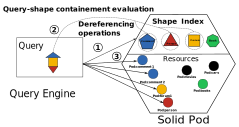
\includegraphics[width=0.50\textwidth]{figure/shape_containement}
    \caption{First, the shape index is dereferenced, 
    then the \emph{query-shape containment} operations are performed in the query engine and lastly, only the relevant resources are dereferenced.}
    \label{fig:shape_index}
\end{figure}
